\section{Modelling of Handover Manipulations}

- present a short version of the deceleration phase (previous paper)
- explain why you decide to resort to this new approach
- show the results of the table of deceleration vs acceleration
- present the new approach of the acceleration phase

  \begin{tikzpicture}
    \draw (0,3)  node[above]{Deformable}  -- (0,-3) node[below]                 {Non-deformable}(-3,0) node[xshift=-6pt,rotate=90] {Non-breakable} -- (3,0)  node[xshift=6pt,rotate=-90] {Breakable};
    \node at (-1.5,1.5) {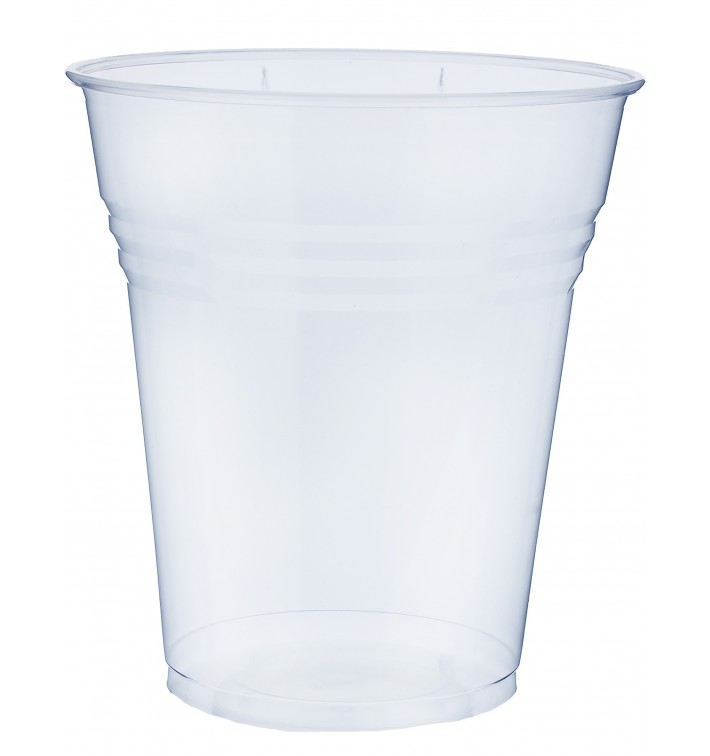
\includegraphics[width = 0.04\textwidth]{Images/transparent_cup.jpg}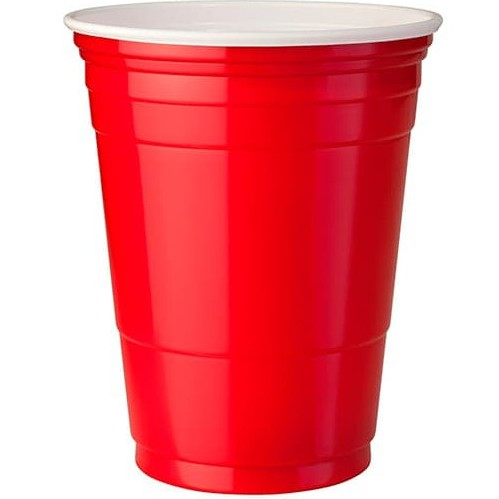
\includegraphics[width = 0.07\textwidth]{Images/red_cup.jpg}};
    \node at (1.5,1.5) {};
    \node at (-1.5,-1.5) {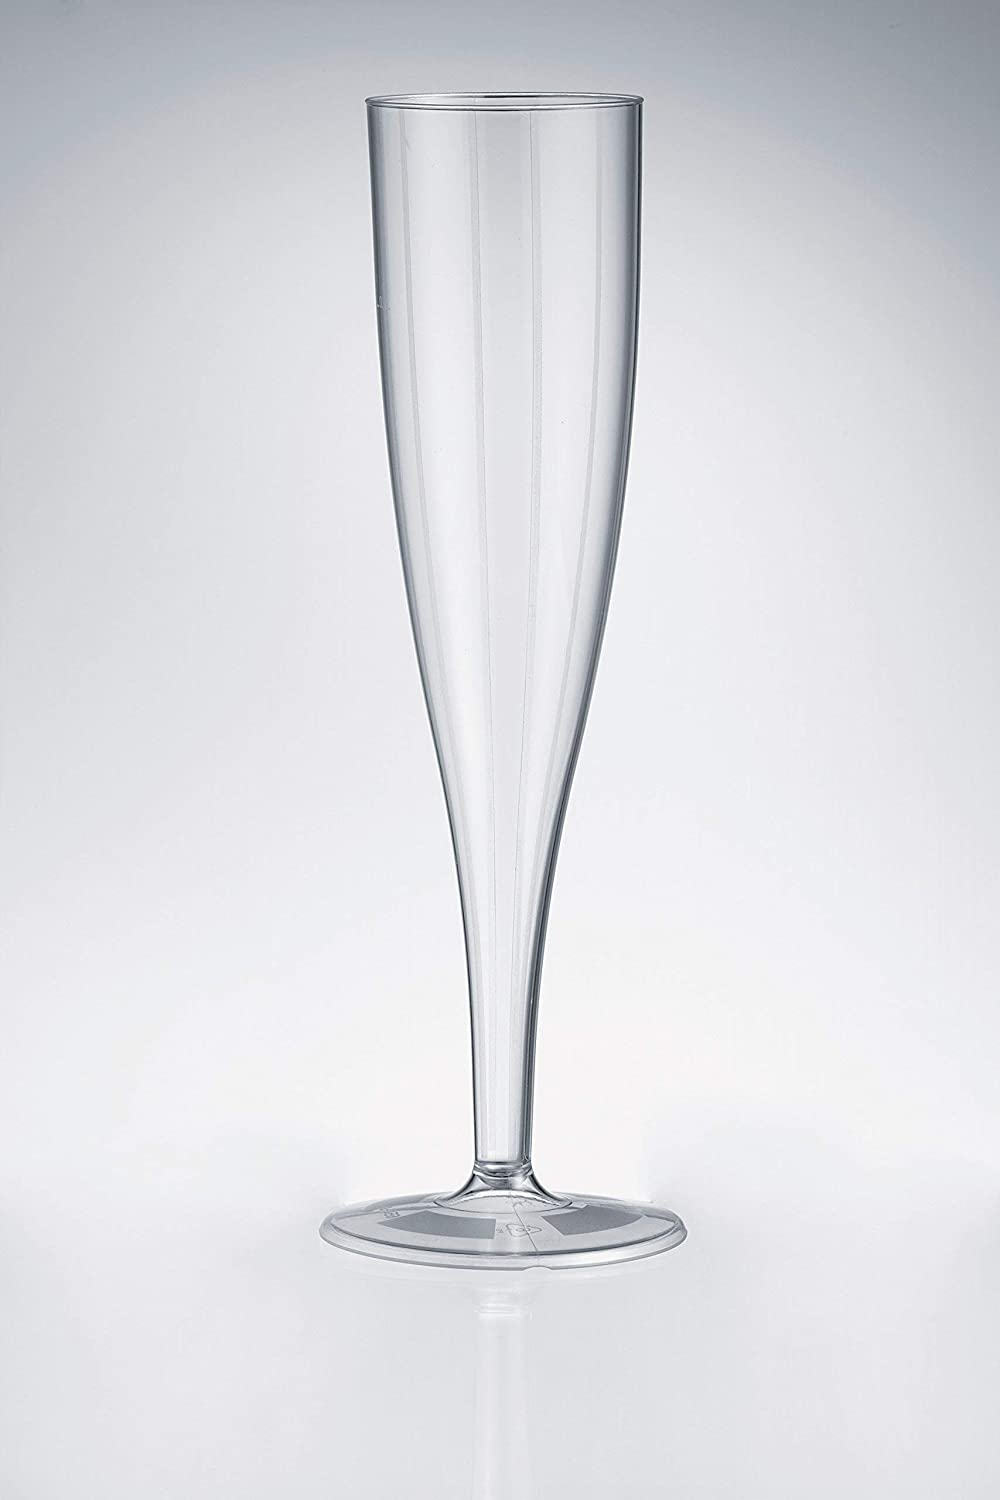
\includegraphics[width = 0.1\textwidth]{Images/champagne_cup.jpg}};
    \node at (1.5,-1.5) {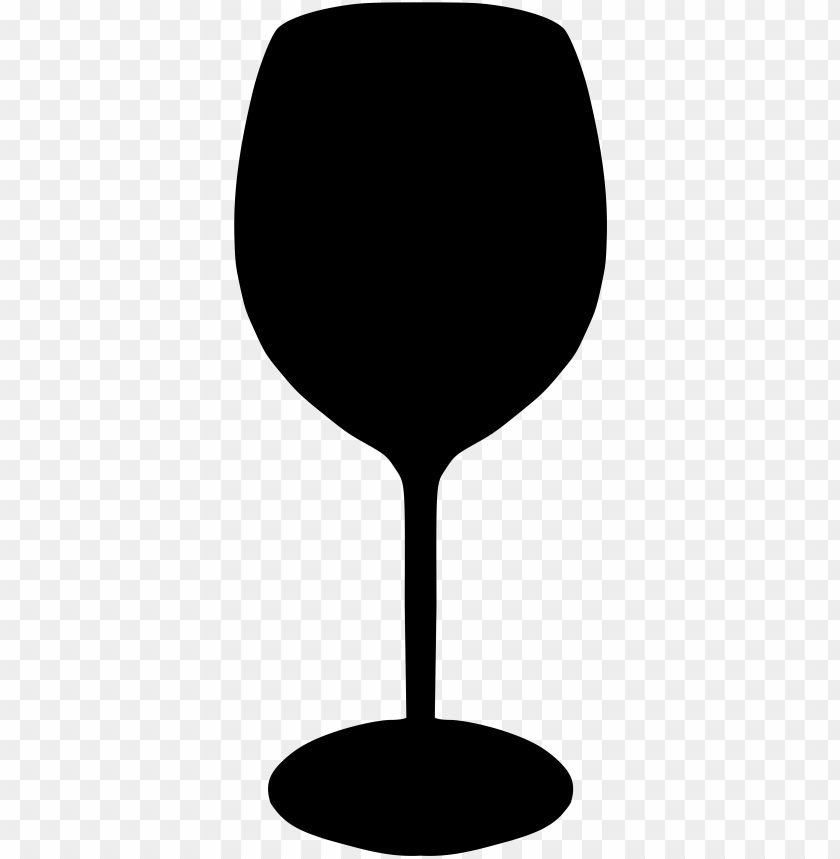
\includegraphics[width = 0.1\textwidth]{Images/wine_glass1.png}};
  \end{tikzpicture}